\begin{frame}{Structure}
	\begin{itemize}
		
		\item \textcolor{gray}{What is a Hidden Markov model?}
		\item \textcolor{gray}{What does \textit{locally stationary} mean?}
		\item Adaptation of a classical consistency proof.
	\end{itemize}
\end{frame}

\section{What is a Hidden Markov Model?}
\begin{frame}{An introductory example}
	\begin{itemize}
		\item Imagine \textbf{A}lice and \textbf{B}ob use a  \textbf{C}hannel for signal transmission.
		\item \textbf{A} sends signals $(X_0, \ldots, X_{n-1})$ where $X_k$ takes values in $\{0,1\}$. 
		\pause 
		\item Channel is noisy and \textbf{B} receives distorted messages $(Y_0, \ldots, Y_{k-1})$, where $Y_k$ also lies in $\{0,1\}$. 
		\item \textbf{B} wants to find out how broken the channel is.
		\pause
		\item The array of signals will be assumed to be a Markov chain, i.\,e. $\P(X_k = i | X_{k-1}, \ldots, X_{0}) =  \P(X_k = i | X_{k-1})$
		\item Transition probabilities $Q_\delta(j,\{i\}) = \P_\delta(X_k = i | X_{k-1}=j)$ are known. 
		\end{itemize}
\end{frame}

\begin{frame}
	Situation can be mathematically modeled in the following way. 
	\begin{itemize}
		\item Consider $(\mathcal{X} := \{0,1\}, \mathcal{B}(\mathcal{X}))$ and  $(\mathcal{Y} := \{0,1\}, \mathcal{B}(\mathcal{Y}))$.
		\item $(X_{k},Y_k)$ is a bivariate Markov chain on $\mathcal{X} \times \mathcal{Y}$ with the following dependence structure.
	\end{itemize}
	\begin{center}
	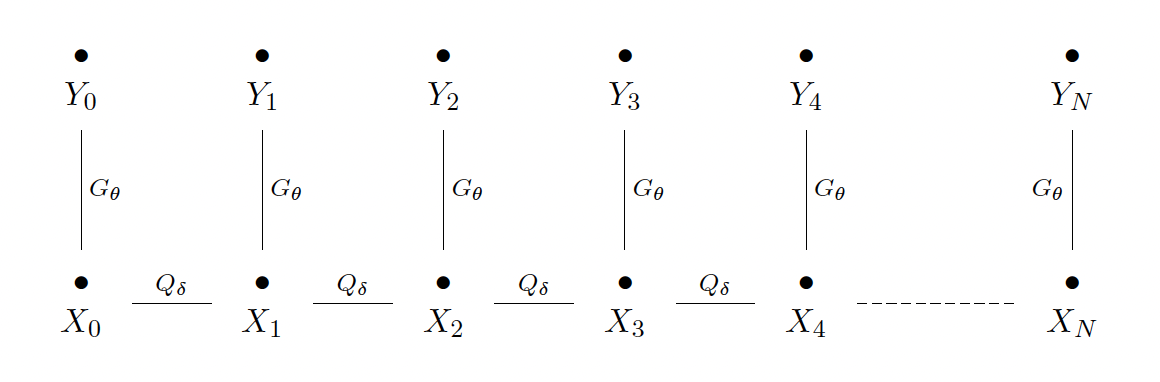
\includegraphics[width=0.8\textwidth]{hmm_structure.png}
	\end{center}
	Say the kernels are represented by the matrices \begin{align*}
		Q_\delta &= \begin{pmatrix}
			Q_\delta(0,0) & Q_\delta(1,0) \\
			Q_\delta(0,1) & Q_\delta(1,1)
		\end{pmatrix} = \begin{pmatrix}
			1-\delta & \delta\\
			\delta& 1-\delta
		\end{pmatrix} \text{ for } \delta \in (0,1) \\ 
	G_\theta &= \begin{pmatrix}
		G_\theta(0,0) & G_\theta(1,0) \\
		G_\theta(0,1) & G_\theta(1,1)
	\end{pmatrix} = \begin{pmatrix}
		1-\theta & \theta \\
		\theta & 1-\theta
	\end{pmatrix}   \text{ for } \theta \in [\delta, 1-\delta] =: \Theta. 
	\end{align*}
\end{frame}

\begin{frame}
\small \begin{align*}
	Q_\delta &= \begin{pmatrix}
		Q_\delta(0,0) & Q_\delta(1,0) \\
		Q_\delta(0,1) & Q_\delta(1,1)
	\end{pmatrix} = \begin{pmatrix}
		1-\delta & \delta\\
		\delta& 1-\delta
	\end{pmatrix} \text{ for } \delta \in (0,1) \\ 
	G_\theta &= \begin{pmatrix}
		G_\theta(0,0) & G_\theta(1,0) \\
		G_\theta(0,1) & G_\theta(1,1)
	\end{pmatrix} = \begin{pmatrix}
		1-\theta & \theta \\
		\theta & 1-\theta
	\end{pmatrix}   \text{ for } \theta \in [\delta, 1-\delta] =: \Theta. 
\end{align*}
\normalsize
\begin{itemize}
 \item \textbf{B} knows $\delta$ and could now resort to the highly developed  theory of \textit{Hidden Markov models} -- for example Maximum likelihood estimation for $\theta \in [\delta, 1- \delta]$.
\item Hidden Markov Models are models of the above form. In the \textit{classical and well-understood} homogeneous case 
\end{itemize}
\begin{center}
	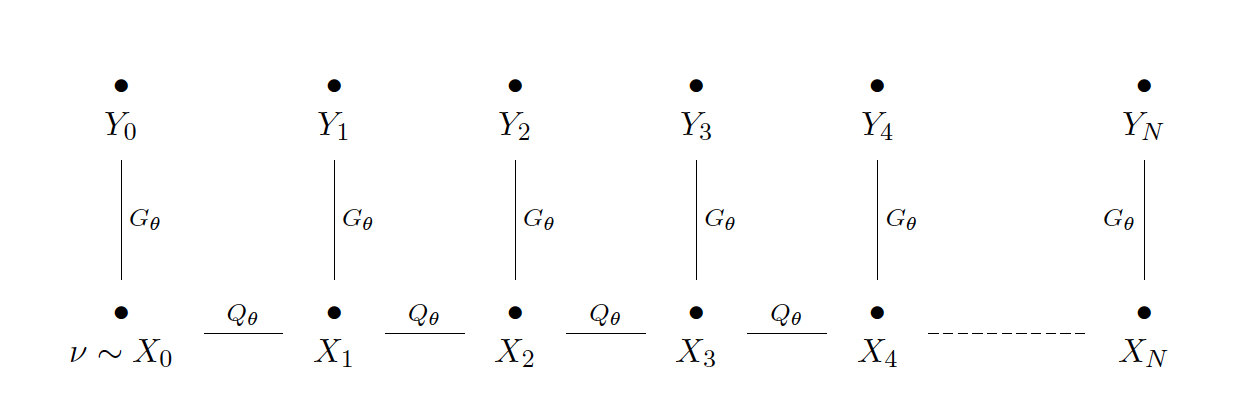
\includegraphics[width=0.8\textwidth]{general_hmm.png}
\end{center}
\end{frame}

\begin{frame}{The formal definition}
	\begin{center}
		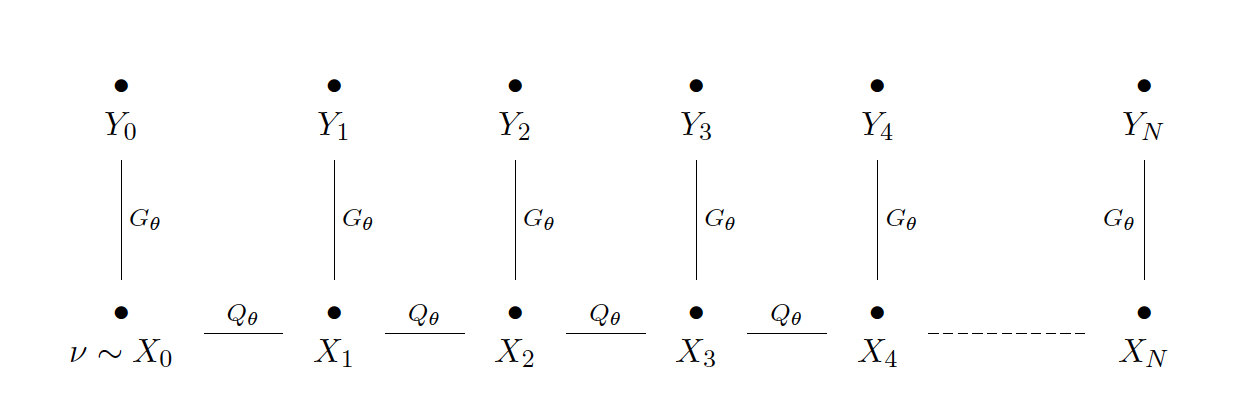
\includegraphics[width=0.7\textwidth]{general_hmm.png}
	\end{center}
	\begin{definitionblockname}{Hidden Markov Models}
Let $(\mathcal{X},\mathcal{A}_\mathcal{X})$ and $(\mathcal{Y},\mathcal{A}_\mathcal{Y})$ be measurable spaces and let $(Z_k)_k = ((X_k, Y_k))_{k}$ be a bivariate Markov chain on $\mathcal{X} \times \mathcal{Y}$. We say that $(Z_k)_k$ is a Hidden Markov Model, if for every $k$ there is a Markov kernel $Q_k$ from  $(\mathcal{X},\mathcal{A}_\mathcal{X})$ to itself and a Markov kernel $G_k$ from $(\mathcal{X},\mathcal{A}_\mathcal{X})$ to $(\mathcal{Y},\mathcal{A}_\mathcal{Y})$ such that for every bounded and measurable $f: \mathcal{X}\times \mathcal{Y} \to \R$ we have \[
\E[f(X_{k},Y_k) | X_0^{k-1}, Y_{0}^{k-1}] = \int_\mathcal{X} \int_\mathcal{Y} f(x,y) G_k(x,dy) Q_k(X_{k-1},dx)
\]
\end{definitionblockname}
\end{frame}

\begin{frame}{Applications of Hidden Markov Models}
	\begin{center}
		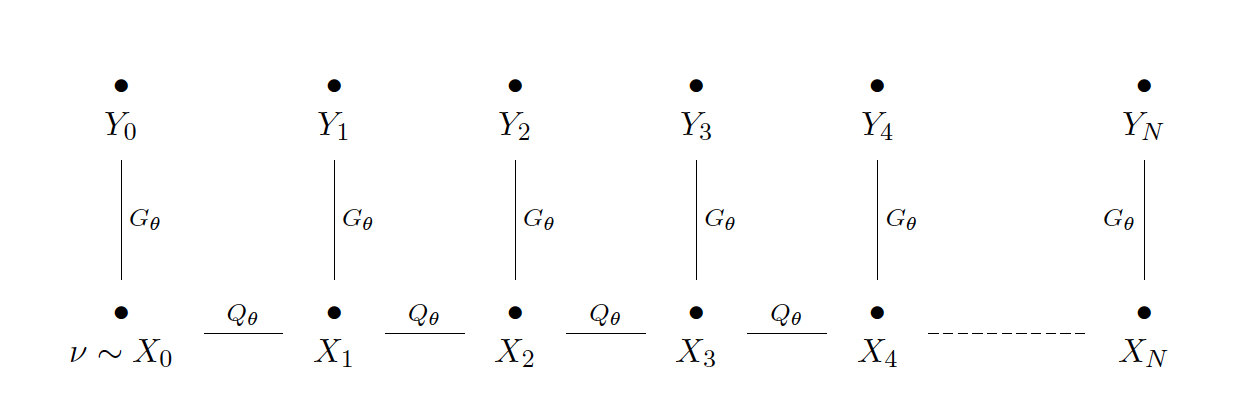
\includegraphics[width=0.8\textwidth]{general_hmm.png}
	\end{center}
\begin{itemize}
	\item Real-world phenomena $X_k$ that are only observed via noisy or incomplete data. 
	\begin{itemize}
		\item physical quantities observed in experiments
		\item evolution of medical indicators whose measurements are noisy
		\item ...
	\end{itemize}
	\item live-tracking of moving objects 
	\item ...
\end{itemize}
\end{frame}
%% Intro locally stationary
\section{What is local stationarity?}
\begin{frame}{The issue of homogeneity and stationarity}
		\begin{center}
		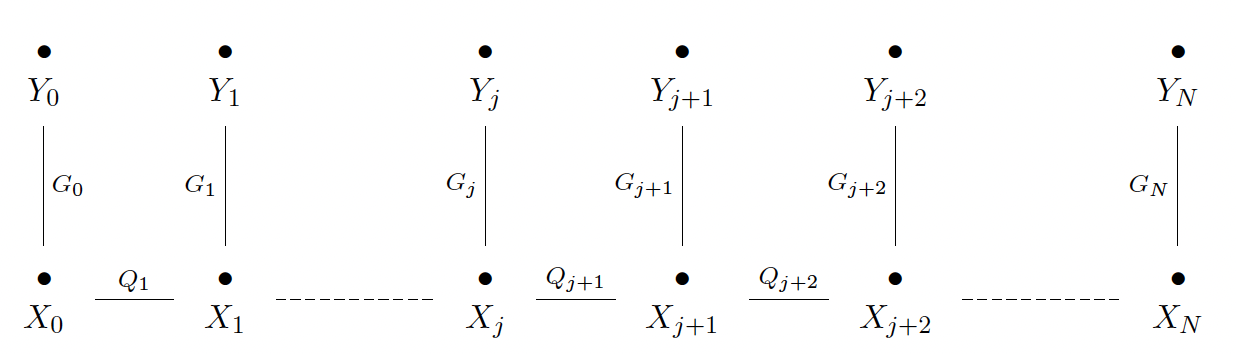
\includegraphics[width=0.8\textwidth]{nonhom_chain.png}
	\end{center}
	\begin{itemize}
	\item Homogeneity/Stationarity is a key requirement for the general consistency results on maximum likelihood estimators to hold. 
	\pause
	\item ... and also to somewhat even make sense.
	\item $\hat{\theta}_N \in \operatorname{argmax}_{\theta \in \Theta}\log \rho_\theta(Y_0^{N})$ not expected to approximate anything useful, if transition parameters evolve \textit{drastically} over time. 
	\end{itemize}
\end{frame}

\begin{frame}
	Typical situation: \begin{itemize}
		\item Provided with an array of $N+1$ many observations $Y_0, \ldots, Y_N$ 
		\item and reasonable to assume transition kernels $Q$ and $G$ are approximately the same around $\lfloor tN\rfloor$  for $\approx bN$ many observations. 
		\item Aim to find out what the kernels around $\lfloor tN \rfloor$ look like. 
		\end{itemize}
\pause		
\begin{center}
	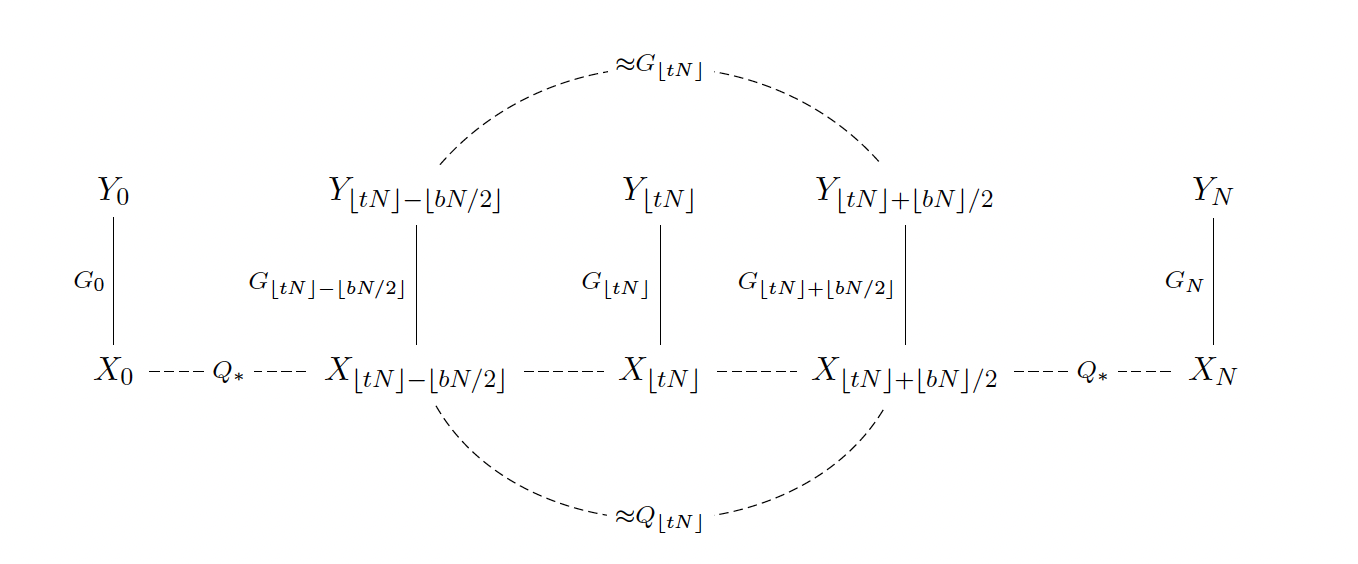
\includegraphics[width=0.8\textwidth]{locally_stationary_idea.png}
\end{center}	
\begin{itemize}
	\item Pretend homogeneity around $\lfloor tN \rfloor$ 
	\item and do maximum likelihood estimation \textit{anyway} only including the observations from that window of size $\approx bN$
\end{itemize}
\end{frame}

\begin{frame}
	In conclusion, consider a maximum likelihood estimator resembling
	\[
	\hat{\theta}_N \in \operatorname{argmax}_{\theta \in \Theta} \log \rho_\theta(Y_{\lfloor tN \rfloor - \lfloor bN / 2 \rfloor}^{\lfloor tN \rfloor + \lfloor bN / 2 \rfloor})
	\] and hope 
	$Q_{\hat{\theta}_N} \approx Q_{k}$ and $G_{\hat{\theta}_N} \approx G_{k}$ for \[k \in [\lfloor tN \rfloor - \lfloor bN / 2 \rfloor, \lfloor tN \rfloor + \lfloor bN / 2 \rfloor] \] \textit{ closely enough.}
	\pause
	\begin{itemize}
	\item Need an \textbf{asymptotic theory} for this estimator (and for other methods of statistical inference as well).
	\pause
	\item In our situation, including more data from $Y_0, \ldots, Y_N$ is \textbf{not an option}. 
	\item I.\,e. no classical asymptotic theory for $\hat{\theta}_n \in \operatorname{argmax}_{\theta \in \Theta} \log \rho_\theta(Y_0^n)$, $n \to \infty$. 
	\end{itemize}
\end{frame}

\begin{frame}{Developing an adequate asymptotic}
	\small
	\[
	\hat{\theta}_N \in \operatorname{argmax}_{\theta \in \Theta} \log \rho_\theta(Y_{\lfloor tN \rfloor - \lfloor bN / 2 \rfloor}^{\lfloor tN \rfloor + \lfloor bN / 2 \rfloor})
	\]
	\normalsize
	\begin{itemize}
		\item Effectively, we estimate a parameter at a point $t \in [0,1]$ in \textit{unit time}. 
		\item Good would be an asymptotic $b \to 0$ but still $bN \to \infty$. 
		\item We get \textbf{both} more stationary around every $t \in [0,1]$ and gather more observations as $N, bN \to \infty$
		\pause 
	\end{itemize}
\small
\begin{definitionblockname}{First (heuristic) definition for local stationarity}
\begin{itemize}
		\item A triangular scheme $\{\{Z_{k,N}\}_{0 \leq k \leq N}\}_{N \geq 0}$ of processes with finite dimensional distributions $\pi_{k,N}^{m,N}$
		\item And for every $t \in [0,1]$ a stationary process $(\widetilde{Z}_{k}(t))_{k \in \Z}$ with finite dimensional distributions $\pi_{k}^m(t) = \pi_{m-k+1}(t)$
		\item $\limsup_{N \to \infty} \sup_{0 \leq k \leq m \leq N, |m-k| \leq l } \norm{\pi_{k}^m(k/N) - \pi_{k,N}^{m,N}}_{TV} = 0 \qquad \;\forall l \geq 1$ 
	\end{itemize}
\end{definitionblockname}
\end{frame}

\begin{frame}
	\small
	\[ \limsup_{N \to \infty} \sup_{0 \leq k \leq m \leq N, |m-k| \leq l } \norm{\pi_{k}^m(k/N) - \pi_{k,N}^{m,N}}_{TV} = 0.\]
	\normalsize
	Of course, variations possible 
	\begin{itemize}
		\item Other metric on the distributions' space possible
		\item And definition involves subtleties (continuity of limit distributions)
		\item Often possible to derive explicit bounds of the form \[
		\norm{\pi_k^m(u) - \pi_{k,N}^{m,N}}_{\text{TV}} \leq C_l \left[\left|u- \frac{k}{N}\right| + \frac{1}{N}\right] \text{ for } 0 \leq m-k \leq l 
		\]
		\pause
		\item \textcolor{gray}{... there will also be other notions}
	\end{itemize}
	\pause
	What does the MLE look like now? Morally at least like
\[
\hat{\theta}_N(t) \in \operatorname{argmax}_{\theta \in \Theta} \log \rho_\theta(Y_{\lfloor tN \rfloor - \lfloor bN / 2 \rfloor, N}^{\lfloor tN \rfloor + \lfloor bN / 2 \rfloor,N})
\]
What happens as $N \to \infty$, $b \to 0$ but yet still $bN \to \infty$?
\end{frame}
